\chapter{Theory}
\section{Terahertz radiation}
The radiation that is produced by the following experiment is Terahertz ($\si{\tera\hertz}$) radiation.
As the name describes its frequency regime lies at about $0.3-30\cdot10^{12}\si{\hertz}$.
Its wavelength can be easily calculated
\begin{equation}
    \lambda = \frac{c}{\nu}
\end{equation}
with the speed of light $c$ and its frequency $\nu$.
Which results in a wavelength of about $\SI{100}{\micro\meter}-\SI{1}{\milli\meter}$.
This means it lies between infrared and microwave radiation.
Terahertz radiation is produced by various non linear effects which only occur at relativly high intensities.
The need of high intensities makes it hard to produce it effiecently.
The result is the so called Terahertz-gap that is slowly being closed by new techniques and advances in science.
Water has the capability to absorb $\si{\tera\hertz}$ radiation, which will be shown later.
%%%%%%%%%%%%%%%%%%%%%%%%%%%%%%%%%%%%%%%%%%%%%%%%%%%%%%%%%%%%%%%%%%%%%%%%%%%%%%%%%%


%%%%%%%%%%%%%%%%%%%%%%%%%%%%%%%%%%%%%%%%%%%%%%%%%%%%%%%%%%%%%%%%%%%%%%%%%%%%%%%%%%
\section{Optical rectification}\label{sec:optic_ref}
To produce $\si{\tera\hertz}$ radiation we take advantage of optical rectification or rather a kind of difference frequency mixing that is very simmilar to optical rectification.
Optical rectification is a second order non linear effect and thus can be just observed in non linear materials.
This effect causes a DC polarization in the crystal that if moduled correctly causes $\si{\tera\hertz}$ radiation.
The DC polarization occurs when an outer electric field interacts with the crystal.
Because of the nonlinear structure and in turn the anharmonic potential of crystal charges, the charges oscillate further into one dircetion then the other.
The displacement of charge is what causes the DC polarization.
To discuss the effect in detail we take a look at the polarization

\begin{equation}
P = \chi(E) E \epsilon_0
\end{equation}

which is directly proportional to the elctric field $E$ and the susceptibilty $\chi(E)$.
Which in turn can be expanded to 

\begin{equation}
    \chi(E) = \chi_0 + \chi_1 E +\chi_2 E^2 + ...   \, .
\end{equation}

As describe earlier optical rectification is a second order effect and describe by the $P_\text{nl} = \chi_2 E^2$ part.
Because the laser produces electro magnetic radiation at a whole bandwith of frequencies $\omega + \Delta\Omega$, in a gaussian profile, its necessary to consider all of those electric fields mixing inside the crystal.
To simplify its best to first take a look at just two electric fields.
One of those electric fields oscillats at frequency $\omega_1$ and the other at frequency $\omega_2$.
The resulting second order polarization term 

\begin{equation}
    P_\text{nl} = \chi_2 \epsilon_0 \frac{E_0^2}{2}\left[cos((\omega_1 - \omega_2)t) + cos((\omega_1 + \omega_2)t)\right]
\label{eq:two_freq_mixing}
\end{equation}

shows a \textbf{cosin} with a diffrence dependency $\omega_1-\omega_2$ and one with a sum dependency $\omega_1+\omega_2$.
The one with the difference dependens results in the production of $\si{\tera\hertz}$ radiation. % the one with the sum depends is important for second harmonic generation
The sum part of equation \eqref{eq:two_freq_mixing} is not important for $\si{\tera\hertz}$ production and will be neglected in further calculations \cite[45--46]{wiki_book}.
If the whole bandwith $\omega + \Delta\Omega$ is now taken into account not just two frequencies mix but all.
This results in a polarization dependency on the bandwith $\Delta\Omega$ as such
\begin{equation}
    P_{\Delta\Omega} = \chi_2 \epsilon_0 \frac{E_0^2}{2}cos(\Delta\Omega t) \, .
\end{equation}
With a bandwith in the femtosecond regime the resulting change in polarization produces $\si{\tera\hertz}$ radiation \cite[289--291]{book_optical_rectification}\cite[46]{wiki_book}.
\\\\
The process $\si{\tera\hertz}$ production can also be explained by the excitation of higher energy levels.
It is visualized in figure \ref{fig:freq_mix}.
\begin{figure}
    \centering
    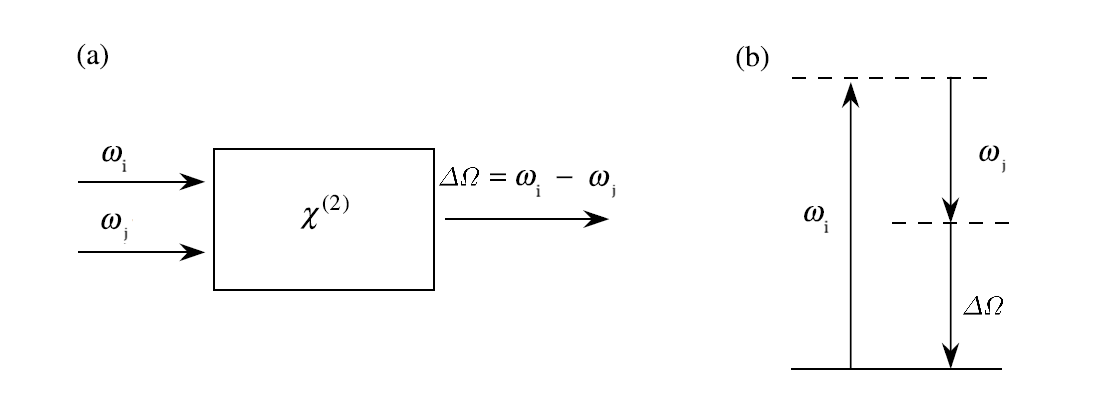
\includegraphics[width=\textwidth]{refferenced_pic/diffrence_frequency_mixing.PNG}
    \caption{Graphic a) shows the two frequencies $\omega_\text{i} $ and $\omega_\text{j}$ going into the nonlinear medium with susceptibilty $\chi_2$.
    Through diffrence frequency mixing the medium emitts radition at frequency $\Delta\Omega$.
    Graphic b) shows the interaction of frequency $\omega_\text{i} $ and $\omega_\text{j}$ inside the medium.
    Here $\omega_\text{i}$ excites a higher virtual energy level, from which $\omega_\text{j}$ gets substracted which leaves $\Delta\Omega$.}
    \label{fig:freq_mix}
\end{figure}
The frequency $\omega_\text{i}$ that goes into the crystal excites a higher energy level.
Now the other frequency $\omega_\text{j}$ that goes into the crystal lowers the energy state again.
Because of the conservation of energy the crystal puts out a photon of the resulting diffrence

\begin{equation}
    \Delta\Omega = \omega_\text{i} - \omega_\text{j} \, .
\end{equation}
%%%%%%%%%%%%%%%%%%%%%%%%%%%%%%%%%%%%%%%%%%%%%%%%%%

%Hier noch Grafik rein und vielleicht nochmal was ändern
%Patrick hat das ganze ja eher durch das anregen von virtuellen Energielevel erklärt.
%Dazu wäre eine Grafik auch gut

%%%%%%%%%%%%%%%%%%%%%%%%%%%%%%%%%%%%%%%%%%%%%%%%%%

\section{Electro-optic sampling}\label{sec:eos}
To detect the $\si{\tera\hertz}$-electric field the electro-optic effect also known as pockels effect is used.
Through this effect a birefringence is induced in the detection crystal which in turn changes the polarization of the probe beam.
The phase shift 
\begin{equation}
    \text{sin}(\theta) = \frac{2\pi}{\lambda} n_0^3 l r E_\text{THz}
\end{equation}
is directly proportional to the electric field. 
It is also proportional to the wavelength $\lambda$, the crystal thickness $l$, the electrooptic coefficient $r$ and the refractive index $n_0$ \cite{wiki_book}. 
Through measurement of the change in polarization it is than possible to determine the intensity of the electric field of the $\si{\tera\hertz}$-pump beam.
For this two photodiodes are used, which measure the probe beam intensity in dependence of its polarization.
It is explained in section \ref{sec:setup} how the beam is split in its two polarization dependent parts.
One photodiode just measures the intensity of the horizontal polarized probebeam $A$ and one the vertical polarized part $B$.
With the normed diffrence 

\begin{equation}
    \frac{A-B}{A+B} = \text{sin}(\theta) = \frac{2\pi}{\lambda} n_0^3 l r E_\text{THz}
    \label{eq:electricfield_A_B}
\end{equation}

it is possible to dertermine the field strength $E_\text{THz}$ \cite[7]{THZ_eltric_field}.
%%%%%%%%%%%%%%%%%%%%%%%%%%%%%%%%%%%%%%%%%%%%%%%%%%%%%%%%%%%%%%%%%%%%%%%%


%%%%%%%%%%%%%%%%%%%%%%%%%%%%%%%%%%%%%%%%%%%%%%%%%%%%%%%%%%%%%%%%%%%%%%%%
\section{Coherence length}
Because the refractive indices of the $\SI{800}{\nano\meter}$ laser pump beam and the produced $\si{\tera\hertz}$ radiation differ from one another, the pulses travel at diffrent speeds inside the crystal.
If the mismatch is too big the effiency of production and detection of $\si{\tera\hertz}$ radiation through the crystals suffers.
The effective length at which the velocity mismatch can be tolerated is called the coherence length

\begin{equation}
    l(\omega_{\si{\tera\hertz}}) = \frac{\pi c}{\omega_{\si{\tera\hertz}} \left | n_\text{opt eff}(\omega_0) - n_{\si{\tera\hertz}}(\omega_{\si{\tera\hertz}})\right |}
\end{equation}

with 

\begin{equation}
    n_{\text{opt eff}} = n_\text{opt}(\omega) - \lambda_\text{opt}\frac{\partial n_\text{opt}}{\partial \lambda}\big{|}_{\lambda_\text{opt}}   
\end{equation}

here c is the velocity of light $\omega_{\si{\tera\hertz}} = \frac{2\pi}{\nu_{\si{\tera\hertz}}}$ is the frequency of $\si{\tera\hertz}$ radiation, $\omega_0$ is the frequency of the laser, $n_{\si{\tera\hertz}}$ is the refractive inidex of $\si{\tera\hertz}$ radiation in the medium, $n_\text{opt}$ is the refractive index of the pump laser wavelength $\lambda_\text{opt}$ and $n_\text{opt eff}$ is the refractive index of the group velocity of the pump laser radiation \cite[3]{coherence_legnth}.
Because the refractive index of $\si{\tera\hertz}$ radiation and $\SI{800}{\nano\meter}$ laser light in ZnTe is very simmilar for $\si{\tera\hertz}$ frequencies up $\SI{2.5}{\tera\hertz}$ \cite{coherence_legnth} the coherence length for those frequencies is long enough for the application in the setup discribed in section \ref{sec:setup}.
The relation between coherence length and $\si{\tera\hertz}$ frequency in ZnTe is shown in figure \ref{fig:coherence_legnth}.

\begin{figure}
    \centering
    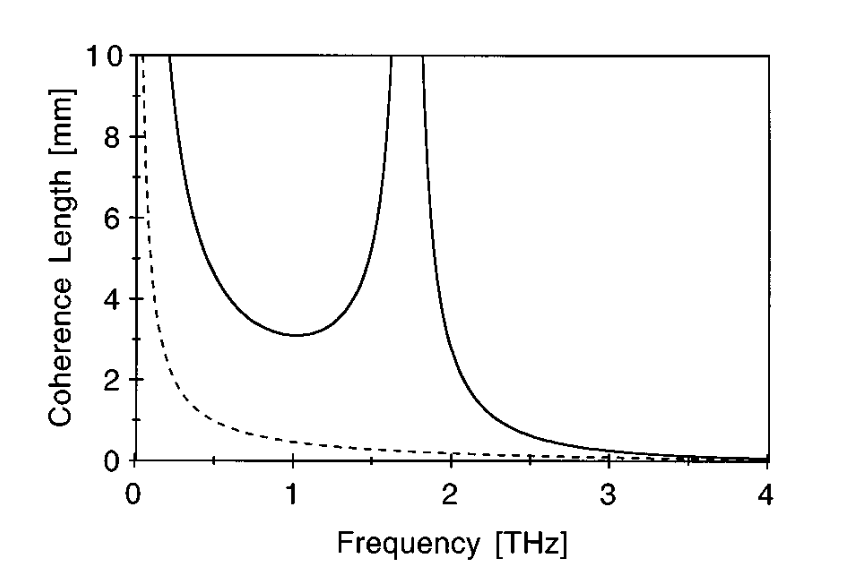
\includegraphics[width=0.5\textwidth]{refferenced_pic/coherence_length_ZnTe.png}
    \caption{The cohenrence length of a $\SI{800}{\nano\meter}$ laser pulse and $\si{\tera\hertz}$ radiation in dependence of the $\si{\tera\hertz}$ frequency.
    The solid line includes the effect of dispersion at optical frequencies. The dotted line neglects the dispersion at optical frequencies.
    The plot was taken from source \cite{coherence_legnth}.}
    \label{fig:coherence_legnth}
\end{figure}

% I need a paper to refernce the coherence length of GaP
\FloatBarrier
\section{Non linear crystals}
Optical non linear crystals exhibit a nonlinearity in there second order susceptibilty $\chi_2$ or in even higher orders.
For this they show special non linear effects at high electric field strengths.
For diffrent purposes diffrent kinds of crystals are in use.
Almost all of these crystals are artificialy produced crystals.
The two crystals that are used in this experiment both show zincblende structure.


\subsection{Zinc telluride}
One of the crystals we use to generate $\si{\tera\hertz}$ radiation is zinc telluride (ZnTe). 
It allows the production of a wideband coherent $\si{\tera\hertz}$ field through means of optical rectification \ref{sec:optic_ref} \cite{ZnTe_Nahata_Weling_1996}.
It should be mentioned that ZnTe has a phonon resonance at $\SI{5.3}{\tera\hertz}$ \cite{phonon_modes} which limits the bandwith of emitted radiation and its ability to detect radiation of that or higher frequencies.
Because optical rectification is a non linear effect it is important to aline the laser to the $<110>$ axis of the crystal.
It is also used as a detection crystal for the $\si{\tera\hertz}$ field.
The ZnTe changes the polarization of the incoming probe beam depedent on the field strength of the $\si{\tera\hertz}$ radiation.
This effect is discussed in section \ref{sec:eos}.

\subsection{Gallium phosphide}
The other crystal that is used to generate $\si{\tera\hertz}$ radiation is Gallium phosphide (GaP).
It is a common emitter of $\si{\tera\hertz}$ radiation with a broad spectrum.
This crystal also exhibits a phonon resonance, but a much higher frequency of about $\SI{11}{\tera\hertz}$ \cite[60]{wiki_book}.
Aswell as ZnTe, Gap needs to stimulated by the laser along its $<110>$ axis.
